\documentclass[a4paper,english]{scrartcl}
\usepackage{amsmath}
\usepackage{graphicx}

\begin{document}

\title{M4P1 Memo}
\maketitle

\section{Surface Elevation Equation [20]}

\subsection{[5]}
Done in the tutorial, all students should have at least 5 points for this section. [5]
\begin{verbatim}
[eta,x,t]=surface_elevation(0.5,16,20)
\end{verbatim}

\begin{figure}
    \centering
    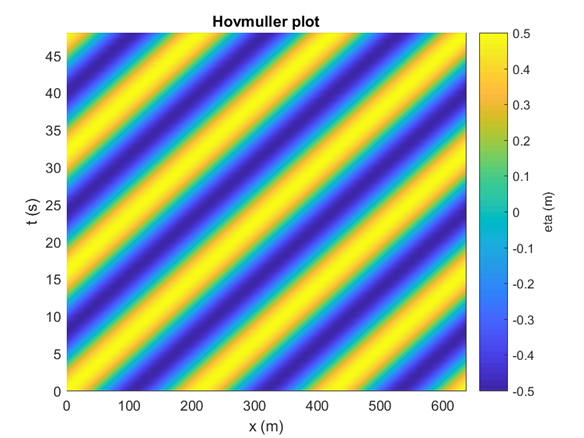
\includegraphics[width=0.7\linewidth]{memo1.png}
\end{figure}

\subsection{[10]}
This is rather simple. Mark down -1.5 for each missing label, etc. [5 for plot, 5 for orbital velocities]

Orbital velocities can be obtained from the figure on page 15, Lecture 3:
\begin{itemize}
    \item At $t = 0$ s – to the right
    \item At $t = 4$ s – downward
\end{itemize}

\section{Dispersion Relation [20]}

(The wavelength of the given wave is 307.8 m.)

\subsection{[10=5+5]}

Most of the code is given, students should have 5 points just from the figure. Visually, it is clear that the maximum wavelength is about 400 m, and this occurs at a water depth of just over 200 m.

\subsection{[10 = 5+5]}



For deep water:
\begin{equation}
    L_0 = \frac{g}{2\pi} T^2 = 399.7 \text{ m}
\end{equation}
\begin{equation}
    d > \frac{L_0}{2} \Rightarrow d > 199.85 \text{ m}
\end{equation}

For shallow water:
\begin{equation}
    L = T \sqrt{g d}
\end{equation}
\begin{equation}
    d < \frac{L}{20} \Rightarrow d < \frac{T^2 g}{400} \Rightarrow d < 6.3 \text{ m}
\end{equation}

The students can write two codes to make the following computations. The error estimate is the same, hence it would be best to put everything in one piece of code or to use the same function. Give 5 only if using a common function (like the \@ handle) for the error estimate, otherwise 4 is max for each component.


\begin{equation}
    L_0 = \frac{g}{2\pi} T^2 = 399.7 \text{ m}
\end{equation}
\begin{verbatim}
    wavelength(16,199.85) = 398.24 m
\end{verbatim}
\begin{equation}
    \text{error} = \frac{\text{estimate} - \text{reference}}{\text{reference}} \times 100 = 0.37\%
\end{equation}

\begin{equation}
    L = T \sqrt{g d} = 125.6
\end{equation}
\begin{verbatim}
    wavelength(16, 6.23) = 123.5 m
\end{verbatim}
\begin{equation}
    \text{error} = 1.68\%
\end{equation}



\end{document}
